\documentclass{article}
\usepackage[T1]{fontenc}
\usepackage{iclr2027_conference,times}
\usepackage{graphicx,booktabs,amsmath,array}
\usepackage[colorlinks=true,linkcolor=black,urlcolor=blue,citecolor=black]{hyperref}
\graphicspath{{../../}}
\iclrfinalcopy
\title{Image-Based 3D Reconstruction\\and Rendering with Gaussian Splatting\\on Ten Objaverse Objects}
\author{Course project group\\Assignment 2 --- 3D Reconstruction and Rendering}
\hypersetup{pdftitle={Assignment 2: 3D Reconstruction and Rendering},pdfauthor={Course project group}}
\begin{document}
\maketitle
\lhead{Assignment 2 --- 3D Reconstruction and Rendering}

\begin{abstract}
We implement and evaluate an image-to-3D reconstruction pipeline on ten textured objects retained by Assignment 1. The pipeline combines calibrated multi-view image generation, SIFT feature matching, COLMAP camera estimation, and Nerfstudio Splatfacto, an implementation of 3D Gaussian Splatting (3DGS). All ten known-camera reconstructions produce genuine model-rendered orbit animations and held-out image evaluations, with mean foreground PSNR of 30.585 dB. Camera recovery remains a separate limitation: only four of ten COLMAP attempts meet an 80\% registration gate, and high coverage does not guarantee accurate poses. A complete estimated-camera pipeline is additionally demonstrated on Cake. Twelve controlled runs on three preselected objects compare view count, input resolution, and training duration. Fewer views yield the largest mean foreground-PSNR decrease in this subset (5.020 dB). Code, complete verified correspondences, animations, commands, and protocol-specific metrics accompany the report.
\end{abstract}

\begin{Form}
\noindent\textbf{Submission information.} Complete the group fields with the actual members and contributions before submission. This coursework uses the ICLR typographic style; it is not an ICLR submission or publication.\par\smallskip
\TextField[name=groupnumber,width=0.77\linewidth,height=0.17in,charsize=9pt,bordercolor={0.65 0.65 0.65}]{Group number: }\par\smallskip
\TextField[name=repositoryurl,width=0.74\linewidth,height=0.17in,charsize=8pt,value={https://github.com/wzw26919/assignment2-3d-reconstruction},bordercolor={0.65 0.65 0.65}]{GitHub repository: }\par\smallskip
\TextField[name=membernames,width=0.75\linewidth,height=0.17in,charsize=9pt,bordercolor={0.65 0.65 0.65}]{Member names: }\par\smallskip
\TextField[name=membercontributions,multiline=true,width=0.69\linewidth,height=0.42in,charsize=9pt,bordercolor={0.65 0.65 0.65}]{Individual contributions: }
\end{Form}

\section{Introduction}
The assignment asks for a complete pipeline from images to a reconstructed 3D representation and novel-view rendering, using objects retained by the preceding data-cleaning assignment. In addition to attractive animations, a useful pipeline must preserve evidence of image correspondences, account for camera-estimation failures, and distinguish measured effects from plausible explanations.

We use 3DGS, which represents a scene using optimized Gaussian primitives and a differentiable splatting renderer \citep{kerbl2023}. The software implementation is Nerfstudio Splatfacto \citep{nerfstudio}. COLMAP supplies SIFT matching, geometric verification, and incremental structure from motion \citep{colmap}. Our contribution is a reproducible course pipeline and an empirical analysis, rather than a new reconstruction algorithm.

The experiments address three questions: (1) can image matching recover sufficiently complete and accurate cameras for these isolated objects; (2) how well does Gaussian reconstruction work when camera error is removed; and (3) how do observation count, image resolution, and optimization time affect rendering quality? We report camera estimation and known-camera rendering as separate protocols throughout.

\section{Data and Image Generation}
\paragraph{Assignment 1 provenance.}
The course Objaverse collection is read from SenseCore AFS. We confirmed access by reading a real GLB and checking its \texttt{glTF} magic, version-2 header, and file length. The source dataset is read without changing its assets or permissions. The final Assignment 1 keep manifest contains 48,824 object UIDs. Its exact path, SHA-256 digest, selected cleaning rows, and selection reasons are preserved in \texttt{configs/objects.json}. Source author, license, and asset URLs are retained in \texttt{artifacts/object\_attribution.json}.

Ten objects are selected before inspecting reconstruction outcomes. Eligibility requires complete cleaning features, successful mesh loading, a base-color texture, no animation or Draco compression, 2,000--150,000 faces, sufficient three-dimensional extent, and GLB size below 25 MB. Within ten predefined name categories, candidates are ranked deterministically by Assignment 1 CLIP object score, texture variation, and UID. These categories are name-based selection groups rather than independently verified semantic annotations. The set includes furniture, vehicles, a shoe, a basket-like vase, a toy camera, food, a bag, a globe, and a guitar.

\paragraph{Calibrated observations.}
Blender 4.0.2 loads each GLB, freezes frame 1, removes imported cameras and lights, centers the world-space bounding box, and scales its longest side to two units while preserving relative object transforms. Three rings at elevations $-20^\circ$, $15^\circ$, and $50^\circ$ each contain 24 azimuths. This yields 72 images per object, or 720 images in total, at $512\times512$ pixels. The camera has a 50 mm lens, a 36 mm sensor, and radius four. Three area lights remain fixed in world coordinates. Cycles uses 32 samples, seed 42, no denoising, and an explicitly white RGB background.

The source GLB generates observations only. Reconstruction training does not receive source mesh surfaces or source mesh points. Actual camera-to-world matrices and normalization parameters are saved in \texttt{capture.json}. Direct Blender turntables are not used as reconstruction GIFs.

\begin{figure}[t]
\centering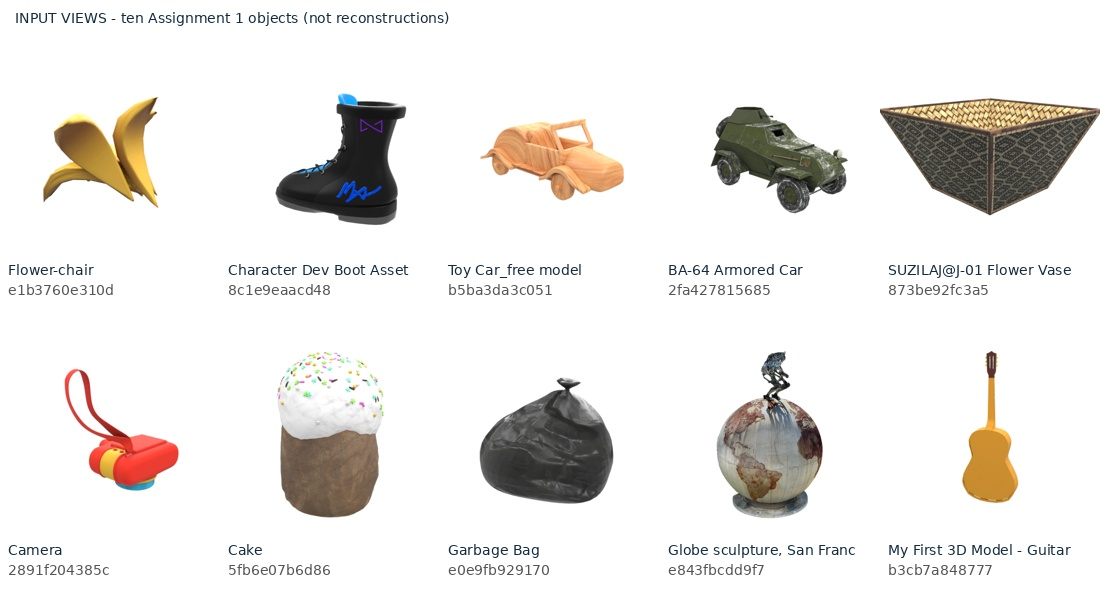
\includegraphics[width=\linewidth]{artifacts/input_contact_sheet.jpg}
\caption{The ten selected objects. Selection is fixed before assessing reconstruction outcomes; all ten remain in the camera-recovery denominator.}
\label{fig:objects}
\end{figure}

\section{Reconstruction Pipeline}
\subsection{Feature matching and camera recovery}
COLMAP 3.9.1 extracts SIFT features on the CPU, exhaustively matches image pairs, and geometrically verifies correspondences. Each 72-image object has up to 2,556 distinct unordered pairs. Exports include all verified feature-index pairs, their keypoint coordinates, image IDs, raw/inlier counts, and eight representative matching plots per object. Plot selection samples low, medium, and high inlier-count pairs rather than displaying only the strongest pair.

The estimated-camera branch runs incremental SfM and bundle adjustment through \texttt{ns-process-data}. Before 3DGS training it requires at least 80\% camera registration and a sparse point cloud. Incomplete or failed attempts retain logs and are not silently replaced. Local pairwise matches constrain two views; a usable camera solution additionally needs a connected and geometrically consistent view graph. This distinction is consequential for weak texture, symmetry, and repeated patterns.

\subsection{Camera and initialization protocols}
\paragraph{Known synthetic cameras (primary ten-object experiment).}
This branch uses the calibrated Blender cameras and initializes 20,000 Gaussians randomly in a two-unit range, without loading source mesh points. Twelve views, at azimuth indices divisible by six across all three elevations, are reserved for evaluation. Their pixels do not enter optimization or initialization. The remaining 60 views train the baseline. This protocol measures appearance reconstruction with known cameras; it does not demonstrate successful camera recovery from images.

\paragraph{Estimated cameras (separate full-pipeline pilot).}
COLMAP estimates cameras and colored sparse points, which initialize Splatfacto. Evaluation images are omitted from the image loss, but they participate in SfM and sparse-point color estimation. Thus they can affect initialization. Metrics from this branch are \emph{transductive diagnostics}, not independent held-out metrics or a direct matched-protocol comparison with the known-camera branch. We completed this branch on Cake and provide its separate reconstructed GIF.

\subsection{Gaussian optimization and animation}
Splatfacto optimizes Gaussian positions, covariance parameters, opacity, and appearance using differentiable rasterization. The primary baseline trains for 15,000 iterations with seed 42 and a white background. Its default progressive schedule starts at 128 pixels, increases to 256 after 3,000 steps, and reaches 512 after 6,000 steps. Estimated-camera training initializes from COLMAP sparse points; known-camera training uses random initialization.

After optimization, \texttt{ns-eval} and the foreground evaluator render evaluation views. Known-camera runs render a continuous 120-frame orbit at $15^\circ$ elevation using \texttt{ns-render camera-path}; the estimated-camera pilot interpolates registered evaluation cameras. These Gaussian-rendered MP4s are converted to 75-frame looping GIFs using a shared palette. All ten main GIFs were checked at four orbit angles for nonblank, stable reconstructions.

\section{Experimental Protocol}
\paragraph{Metrics.}
We record PSNR, SSIM, and LPIPS against target views. We additionally measure foreground PSNR over target pixels whose maximum absolute RGB difference from white exceeds 0.08. Full-frame scores may be inflated by the white background; the foreground approximation may omit white object regions. It therefore complements visual inspection rather than supplying a complete silhouette or geometry metric.

\paragraph{Controlled comparisons.}
Flower-chair, BA-64 Armored Car, and Cake were preselected for the ablations. For each object we train four known-camera runs: a fixed-resolution reference and three interventions (Table~\ref{tab:protocol}). This gives 12 additional controlled runs, including three reference runs. All comparisons use the same twelve evaluation views. For the fewer-view run, 36 candidate views contain 24 training views and these twelve targets.

\begin{table}[t]
\caption{Training protocols. Progressive downscaling is disabled in every controlled comparison. The main ten-object baseline is reported separately.}
\label{tab:protocol}\centering\small
\begin{tabular}{lrrrr}
\toprule
Variant & Input size & Candidate views & Train views & Steps\\
\midrule
Main baseline & $512^2$ & 72 & 60 & 15,000\\
Fixed-resolution reference & $512^2$ & 72 & 60 & 15,000\\
Fewer views & $512^2$ & 36 & 24 & 15,000\\
Lower resolution & $256^2$ & 72 & 60 & 15,000\\
Shorter training & $512^2$ & 72 & 60 & 3,000\\
\bottomrule
\end{tabular}
\end{table}

The fixed-resolution reference prevents the 3,000-step comparison from also changing effective training resolution. Controlled predictions are resampled to the same original $512\times512$ targets for supplementary PSNR, so resolution comparisons evaluate identical pixels. Native Nerfstudio scores remain at each run's own resolution and are labeled separately. All runs use one seed. There are 23 completed trained models in total: ten primary models, twelve controlled models, and one estimated-camera pilot.

\section{Results and Analysis}
\subsection{Ten-object reconstruction and camera estimation}
All ten known-camera baselines complete training, evaluation, and animation export. Mean foreground PSNR is 30.585 dB, with a range of 22.527--33.557 dB. Native full-frame PSNR ranges from 26.524 dB for the basket-like Flower Vase to 42.761 dB for Guitar (Table~\ref{tab:results}). The foreground/background distinction changes how these scores should be interpreted.

\begin{table}[t]
\caption{Primary known-camera rendering results. Reg. is the separate COLMAP registration count, not the camera source used for these rendering metrics. PSNR values are in dB. SSIM is higher-is-better and LPIPS is lower-is-better.}
\label{tab:results}\centering\small
\begin{tabular}{lrrrrr}
\toprule
Object & Reg. & PSNR & SSIM & LPIPS & FG PSNR\\
\midrule
Flower-chair & 2/72 & 41.238 & 0.985 & 0.015 & 33.557 \\
Boot & 28/72 & 38.425 & 0.990 & 0.011 & 30.722 \\
Toy car & 24/72 & 40.667 & 0.983 & 0.019 & 32.165 \\
BA-64 Armored Car & 62/72 & 38.014 & 0.986 & 0.010 & 30.587 \\
Flower Vase / basket & 72/72 & 26.524 & 0.872 & 0.071 & 22.527 \\
Camera & 2/72 & 41.759 & 0.994 & 0.004 & 32.493 \\
Cake & 72/72 & 38.760 & 0.976 & 0.024 & 31.667 \\
Garbage Bag & 24/72 & 33.934 & 0.947 & 0.046 & 28.589 \\
Globe sculpture & 72/72 & 39.283 & 0.990 & 0.009 & 32.792 \\
Guitar & 3/72 & 42.761 & 0.995 & 0.003 & 30.754 \\
\bottomrule
\end{tabular}
\end{table}

Only four of ten COLMAP attempts pass the predefined 80\% registration gate: Armored Car, Flower Vase, Cake, and Globe. Counts range from 2 to 72 registered views. The denominator includes every attempted object, including incomplete reconstructions. Successful feature matching alone therefore does not establish a complete image-to-camera pipeline.

Coverage is also insufficient to establish pose accuracy. Flower Vase registers 72/72 cameras but has median rotation error $32.173^\circ$ after similarity alignment. In contrast, the corresponding errors for Armored Car, Cake, and Globe are $0.538^\circ$, $0.254^\circ$, and $0.129^\circ$. Repeated surface patterns are a plausible explanation for the vase's ambiguous correspondences, not a separately isolated causal finding. Per-object inlier counts, camera coverage, aligned errors, and sparse models accompany the report.

Even with correct cameras, the Flower Vase's reconstructed evaluation images lose fine surface detail and have the lowest foreground PSNR. High-frequency texture and limited representation or optimization capacity are plausible contributors. Known cameras remove one failure mode; they do not guarantee perfect appearance reconstruction or complete hidden-surface geometry.

The Cake estimated-camera pilot completes COLMAP-to-3DGS training and produces its own animation. Its diagnostic PSNR is 35.665 dB, SSIM is 0.9728, and LPIPS is 0.0295. Because target images contribute to SfM and colored initialization, these numbers must not be treated as an independent held-out comparison with the primary experiment.

\subsection{Effects of view count, resolution, and training time}
Across the three preselected objects, fewer views decrease foreground PSNR by 5.020 dB on average relative to the fixed-resolution reference. Per-object changes range from $-5.599$ to $-4.496$ dB. Lower input resolution changes foreground PSNR by $-2.533$ dB on average, with a range of $-4.666$ to $+0.322$ dB. Shorter training changes it by $-2.582$ dB on average, ranging from $-4.794$ to $-1.324$ dB.

\begin{figure}[t]
\centering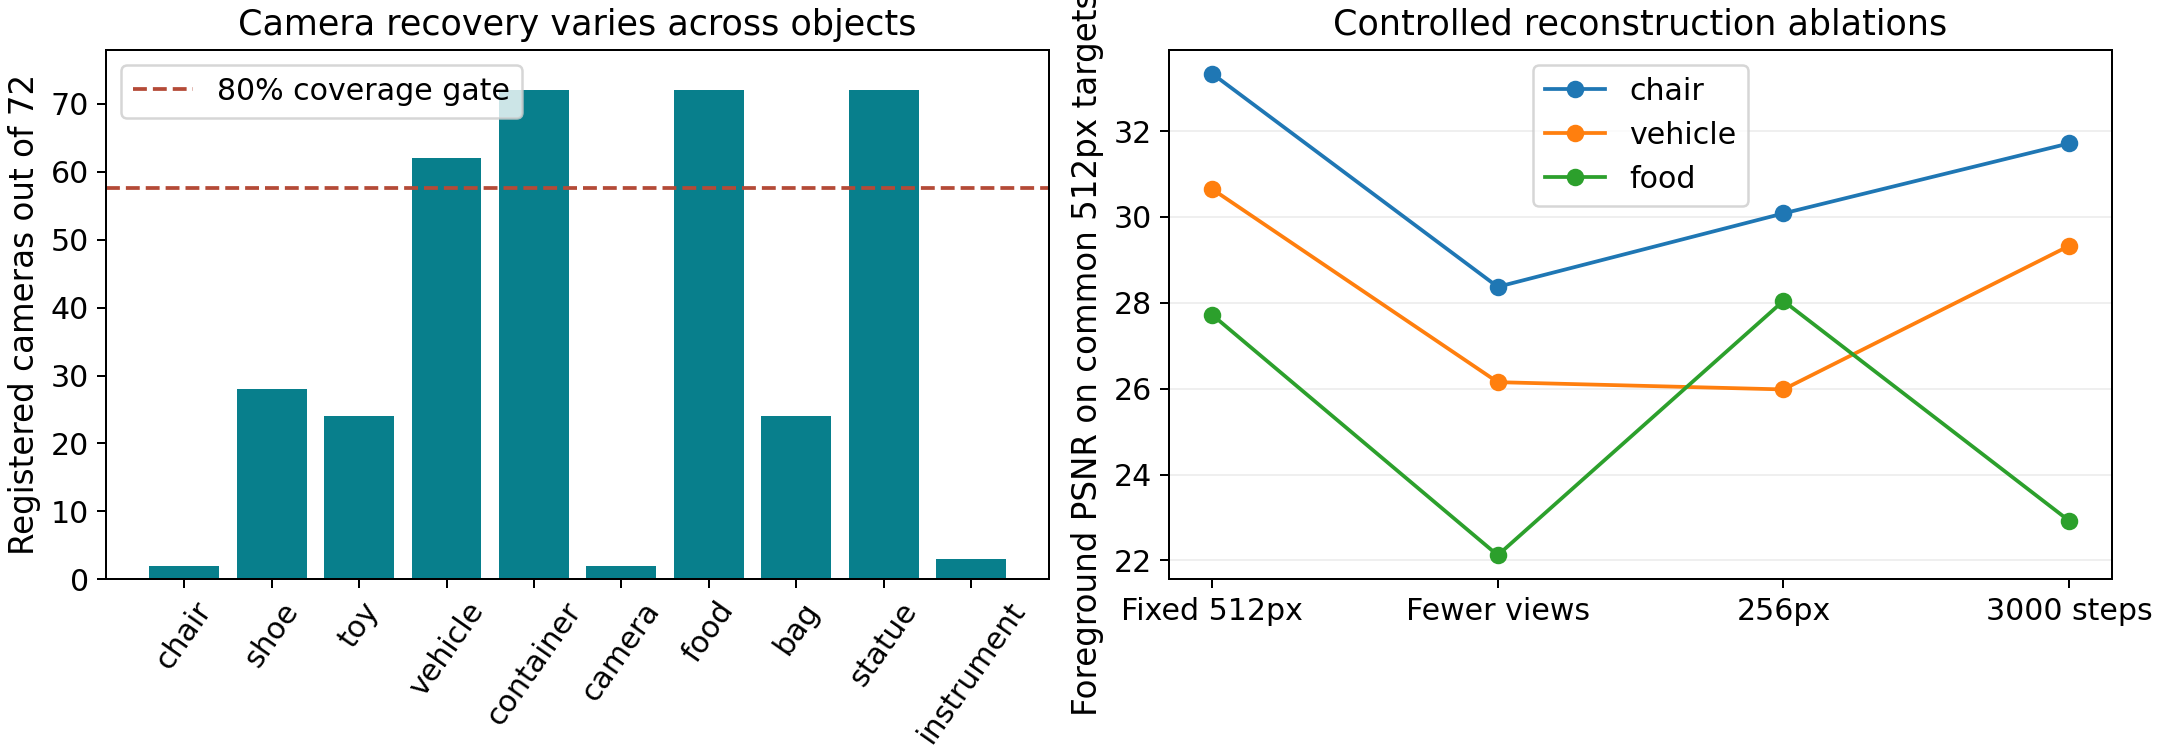
\includegraphics[width=\linewidth]{artifacts/experiment_comparison.png}
\caption{Controlled foreground-PSNR changes against the separate fixed-resolution reference. Every comparison shares the same evaluation views and original 512-pixel target grid. These results describe one seed on three objects.}
\label{fig:ablations}
\end{figure}

Within this subset, reducing observations causes the largest mean degradation among the three tested interventions. This supports prioritizing sufficient views and overlap in this configuration. The small positive resolution change on Cake prevents a universal claim that lower resolution always worsens the result. A single seed and three objects do not establish an ordering that generalizes to all Objaverse assets.

\section{Limitations and Conclusions}
The pipeline produces complete known-camera reconstructions and real 3DGS-rendered animations for ten objects, with point-matching evidence and controlled comparisons. Camera recovery is the clearest observed upstream bottleneck: it frequently lacks coverage and can remain inaccurate even at full coverage. Downstream rendering also depends on available views, detail scale, and optimization budget.

The inputs are synthetic with fixed lighting and limited elevation coverage. There is one random seed, a small ablation subset, and an approximate foreground mask. Image agreement does not prove correct topology or unseen-surface geometry. The estimated-camera pilot uses transductive geometry/color initialization and cannot establish independent generalization. These limits are retained alongside successful outcomes rather than hidden by selective reporting.

\section{Reproducibility, Attribution, and AI Assistance}
The repository contains orchestration and analysis code, dependency versions, actual command lines and timings, camera splits, all verified matching arrays, plots, per-object metrics, and GIF/MP4 animations. Portable correspondences include NPZ arrays, image IDs, keypoint coordinates, and pair-count CSVs. Experiments with identical inputs reference shared matching files explicitly. The offline \texttt{index.html} gallery links the ten main reconstructions and matching examples.

Source GLBs, full descriptor databases, raw capture images, and training checkpoints remain in SenseCore AFS rather than the portable repository. The README documents environment setup, reproduction, failure recovery, and packaging. Six unit tests cover GLB access/header checks, match-pair direction/export, common disjoint evaluation views, orbit geometry, and camera alignment; numerical and visual results additionally come from the actual GPU runs.

Source models retain their original author and license attribution. The group must supply its actual membership and individual contributions in the fields on the first page. Codex assisted with implementation, environment setup, tests, documentation, and tool operation. Assignment-specific user messages and the prompt inventory are included in \texttt{prompts/}; numerical reconstruction does not use language-model or image-generation prompts to fabricate observations or measurements.

\begin{thebibliography}{9}
\bibitem[Kerbl et~al.(2023)]{kerbl2023}
Bernhard Kerbl, Georgios Kopanas, Thomas Leimk\"uhler, and George Drettakis.
3D Gaussian Splatting for Real-Time Radiance Field Rendering.
\emph{ACM Transactions on Graphics}, 42(4), 2023.
\url{https://repo-sam.inria.fr/fungraph/3d-gaussian-splatting/}.
\bibitem[COLMAP contributors(2026)]{colmap}
COLMAP contributors. \emph{COLMAP documentation}. Software version used: 3.9.1.
\url{https://colmap.github.io/}. Accessed 2026.
\bibitem[Nerfstudio contributors(2026)]{nerfstudio}
Nerfstudio contributors. \emph{Splatfacto documentation and Nerfstudio source}.
Software version used: 1.1.5.
\url{https://docs.nerf.studio/nerfology/methods/splat.html};
\url{https://github.com/nerfstudio-project/nerfstudio/tree/v1.1.5}. Accessed 2026.
\end{thebibliography}

\appendix
\clearpage\section*{Reconstruction and matching evidence (1/3)}
Each object shows a held-out target (left) and a trained 3DGS rendering (right), followed by an actual geometrically verified matching pair. Full correspondences and looping GIFs are in the repository.\par\medskip\noindent\begin{minipage}[t]{0.48\linewidth}
\textbf{Flower-chair}\par\smallskip
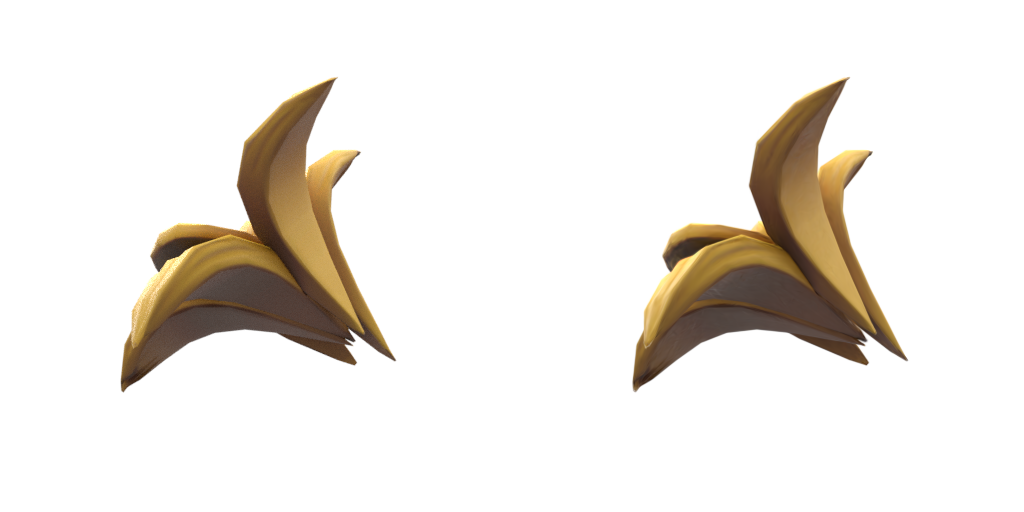
\includegraphics[width=\linewidth]{results/e1b3760e310d4a759cde3146edf40212/evaluation/view_000.png}\par
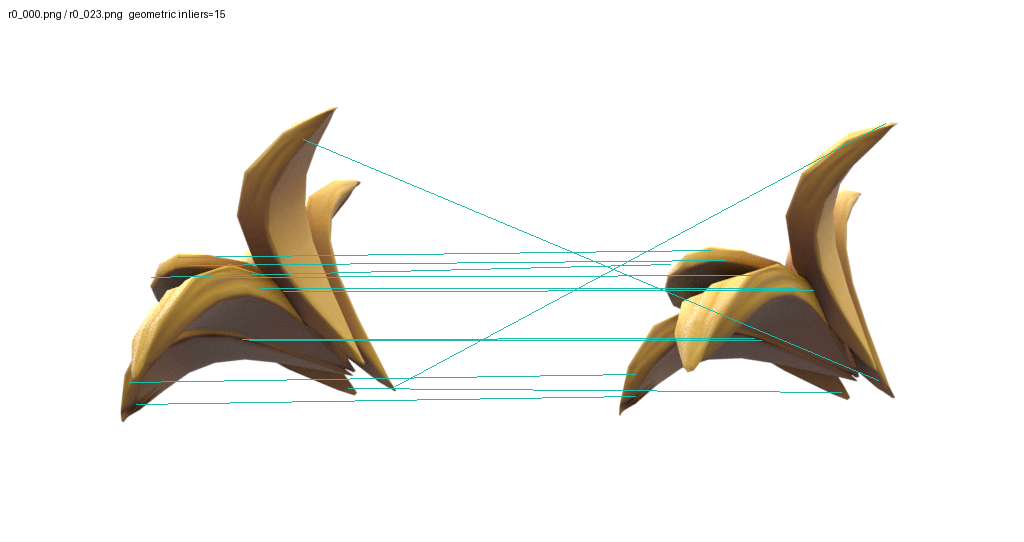
\includegraphics[width=\linewidth]{results/e1b3760e310d4a759cde3146edf40212/matches/matches_00.png}\par
{\footnotesize PSNR 41.24 dB; foreground 33.56 dB.}\end{minipage}\hfill
\noindent\begin{minipage}[t]{0.48\linewidth}
\textbf{Character Dev Boot Asset}\par\smallskip
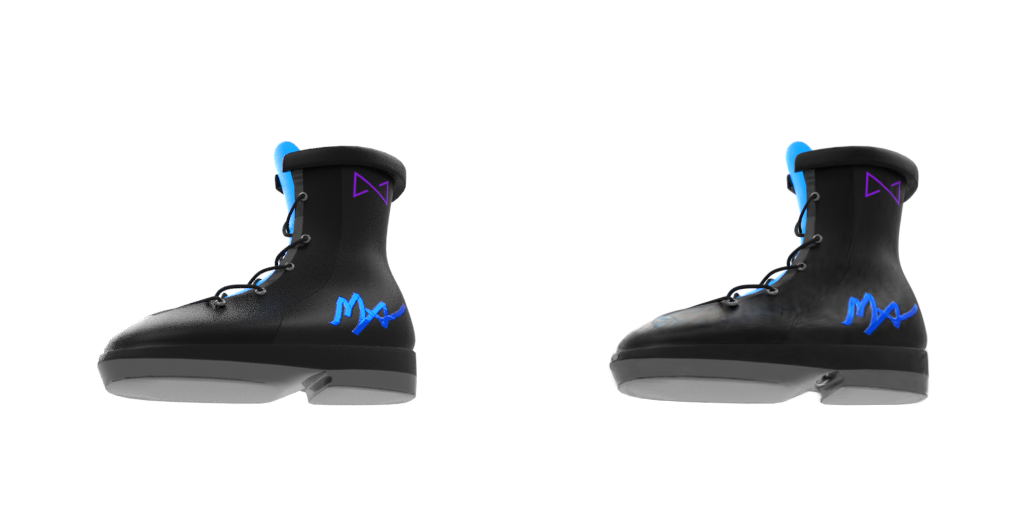
\includegraphics[width=\linewidth]{results/8c1e9eaacd48441f9b356cd2d6c0ba63/evaluation/view_000.png}\par
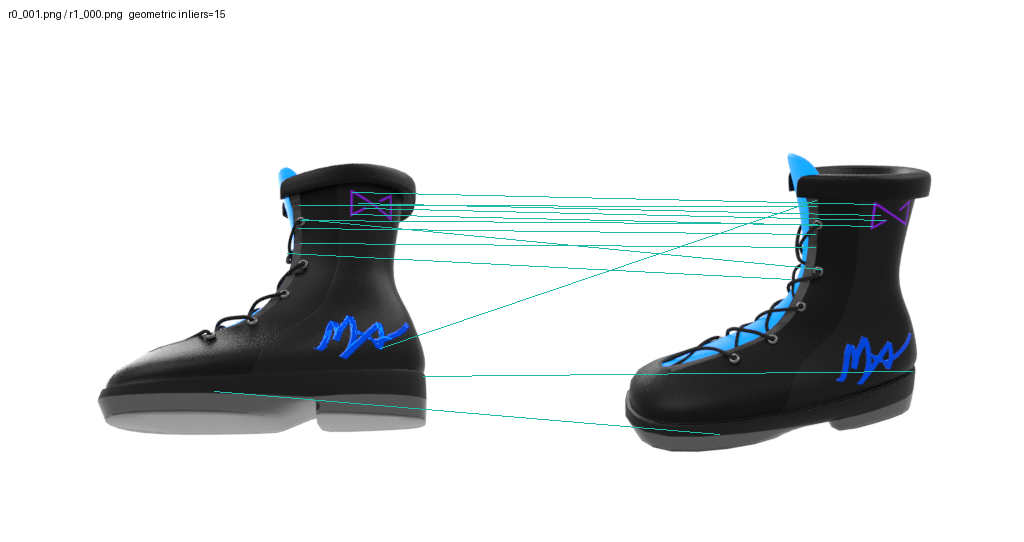
\includegraphics[width=\linewidth]{results/8c1e9eaacd48441f9b356cd2d6c0ba63/matches/matches_00.png}\par
{\footnotesize PSNR 38.43 dB; foreground 30.72 dB.}\end{minipage}\hfill
\par\bigskip
\noindent\begin{minipage}[t]{0.48\linewidth}
\textbf{Toy Car\_free model}\par\smallskip
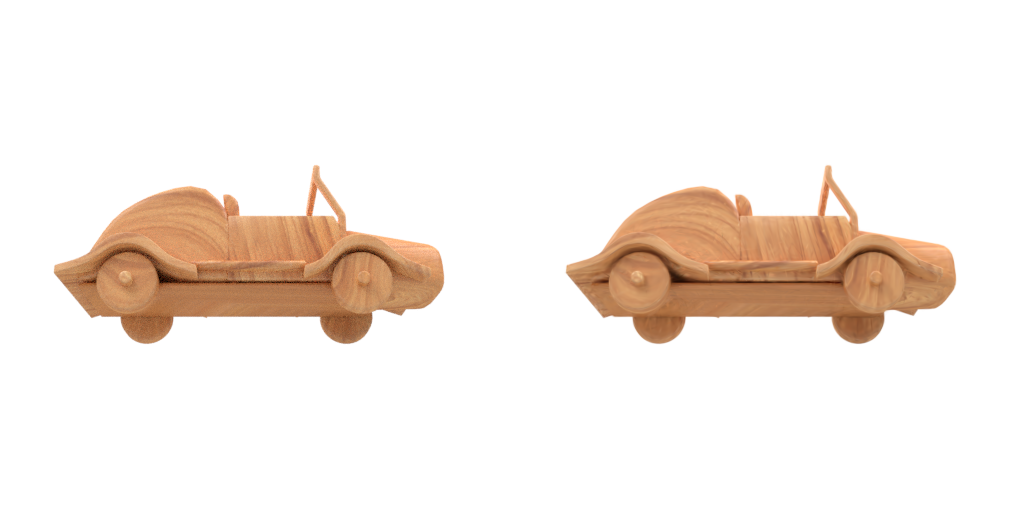
\includegraphics[width=\linewidth]{results/b5ba3da3c0514d938728c2773cb836d2/evaluation/view_000.png}\par
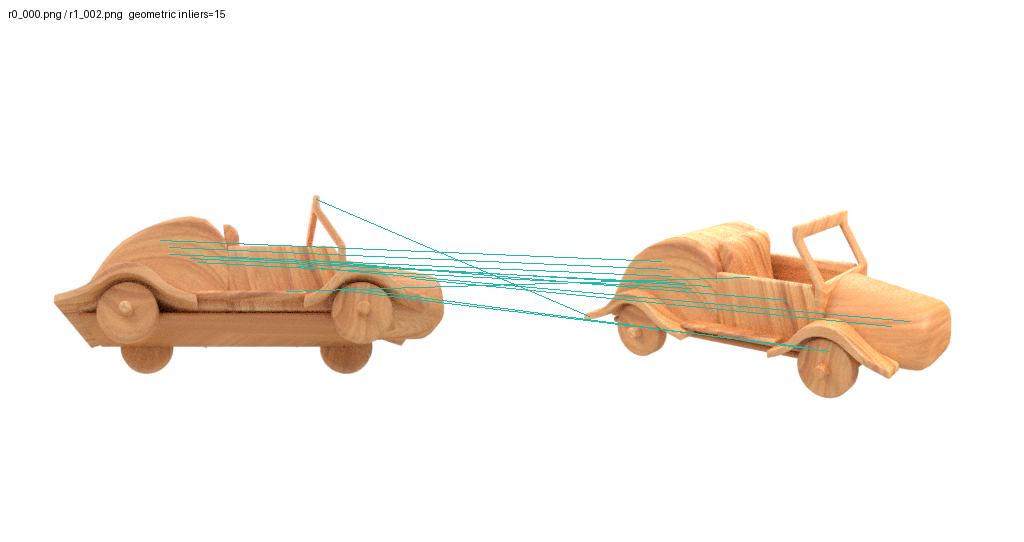
\includegraphics[width=\linewidth]{results/b5ba3da3c0514d938728c2773cb836d2/matches/matches_00.png}\par
{\footnotesize PSNR 40.67 dB; foreground 32.17 dB.}\end{minipage}\hfill
\noindent\begin{minipage}[t]{0.48\linewidth}
\textbf{BA-64 Armored Car}\par\smallskip
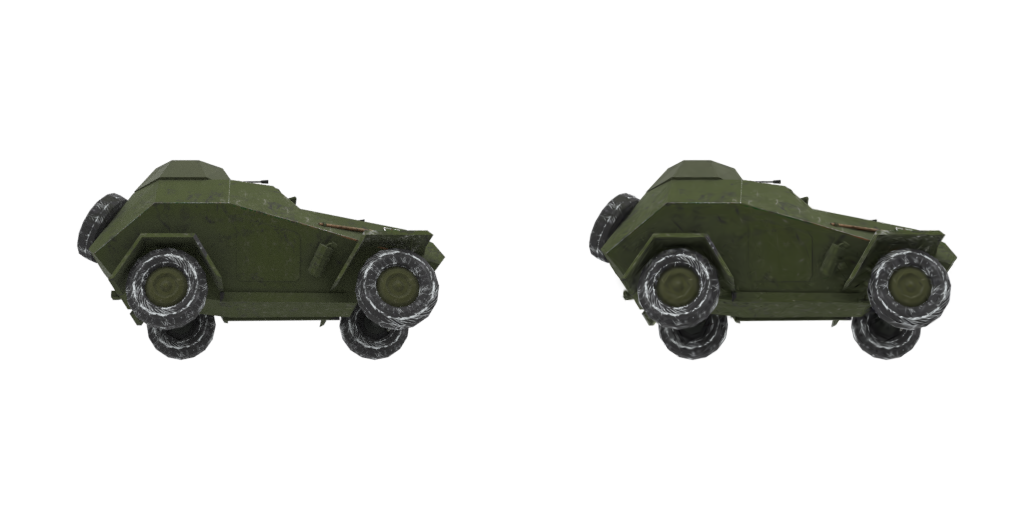
\includegraphics[width=\linewidth]{results/2fa42781568549c0861769cbf51d88fc/evaluation/view_000.png}\par
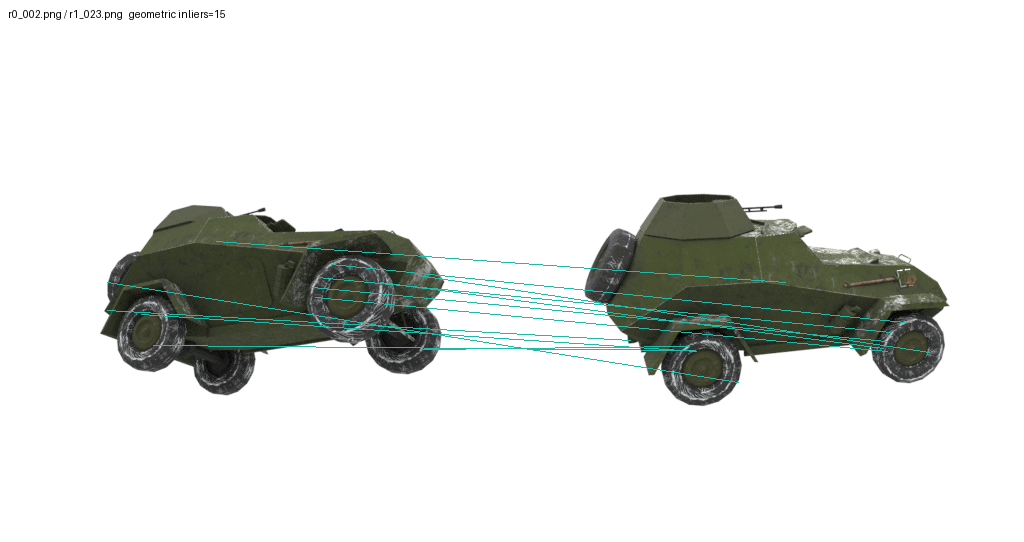
\includegraphics[width=\linewidth]{results/2fa42781568549c0861769cbf51d88fc/matches/matches_00.png}\par
{\footnotesize PSNR 38.01 dB; foreground 30.59 dB.}\end{minipage}\hfill
\par\bigskip
\clearpage\section*{Reconstruction and matching evidence (2/3)}
Each object shows a held-out target (left) and a trained 3DGS rendering (right), followed by an actual geometrically verified matching pair. Full correspondences and looping GIFs are in the repository.\par\medskip\noindent\begin{minipage}[t]{0.48\linewidth}
\textbf{SUZILAJ@J-01 Flower Vase}\par\smallskip
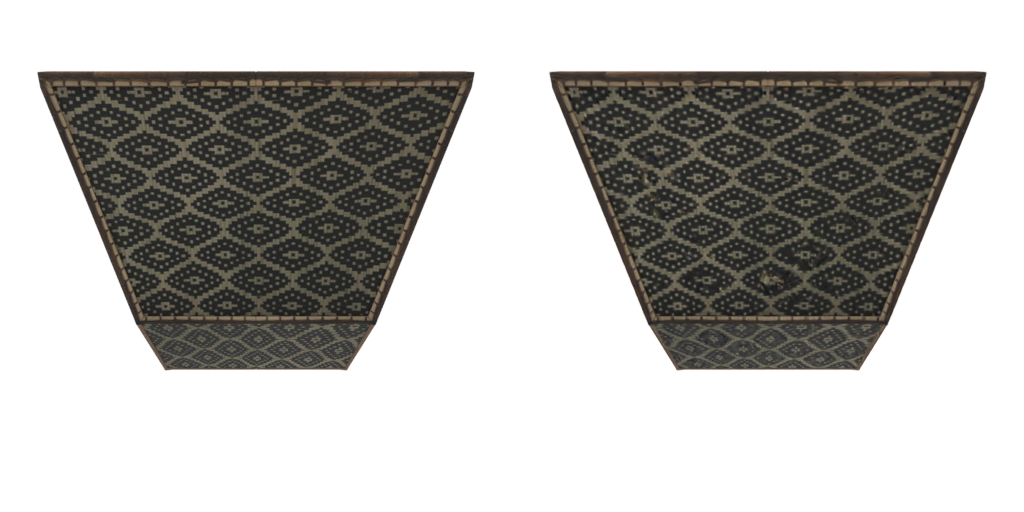
\includegraphics[width=\linewidth]{results/873be92fc3a54d65bac955231029589b/evaluation/view_000.png}\par
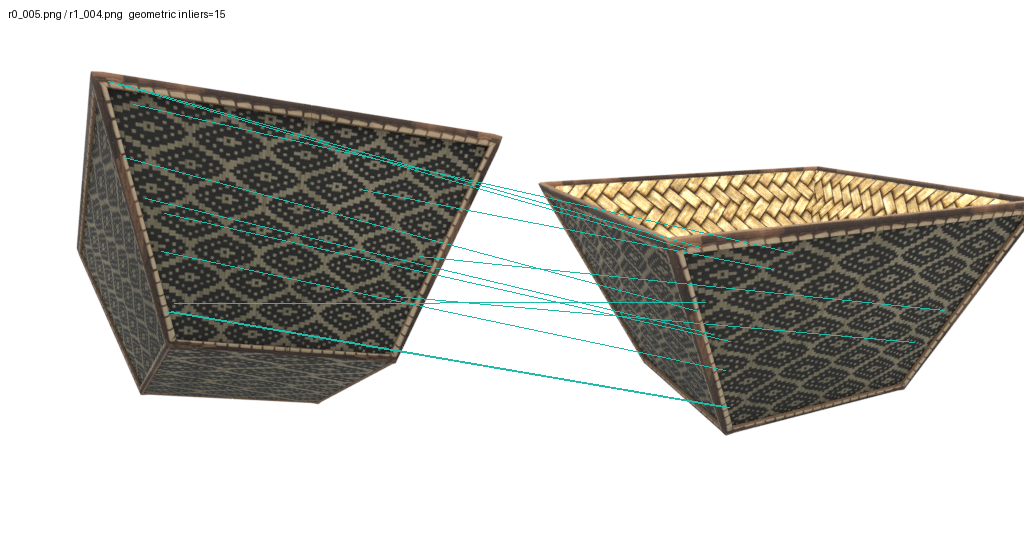
\includegraphics[width=\linewidth]{results/873be92fc3a54d65bac955231029589b/matches/matches_00.png}\par
{\footnotesize PSNR 26.52 dB; foreground 22.53 dB.}\end{minipage}\hfill
\noindent\begin{minipage}[t]{0.48\linewidth}
\textbf{Camera}\par\smallskip
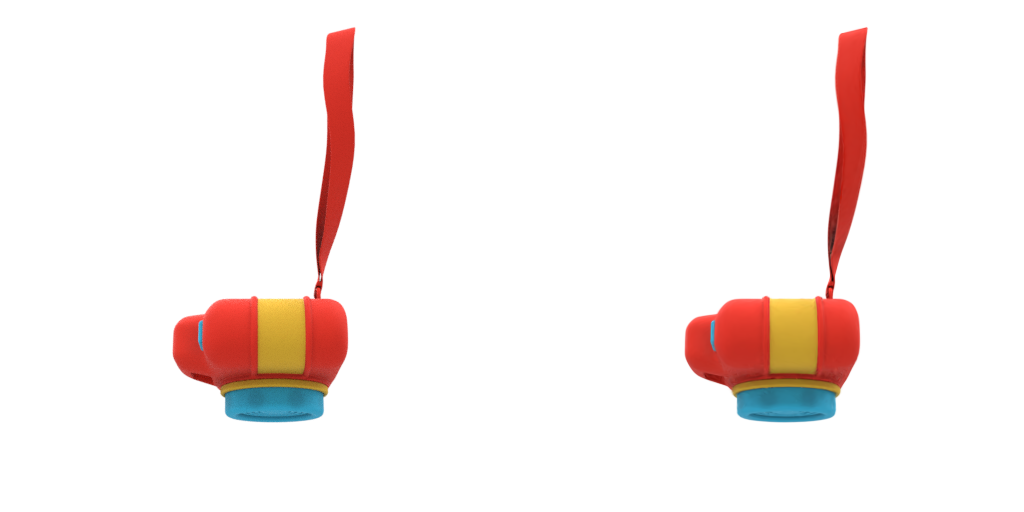
\includegraphics[width=\linewidth]{results/2891f204385c429eb8ab3cbc28bdf36a/evaluation/view_000.png}\par
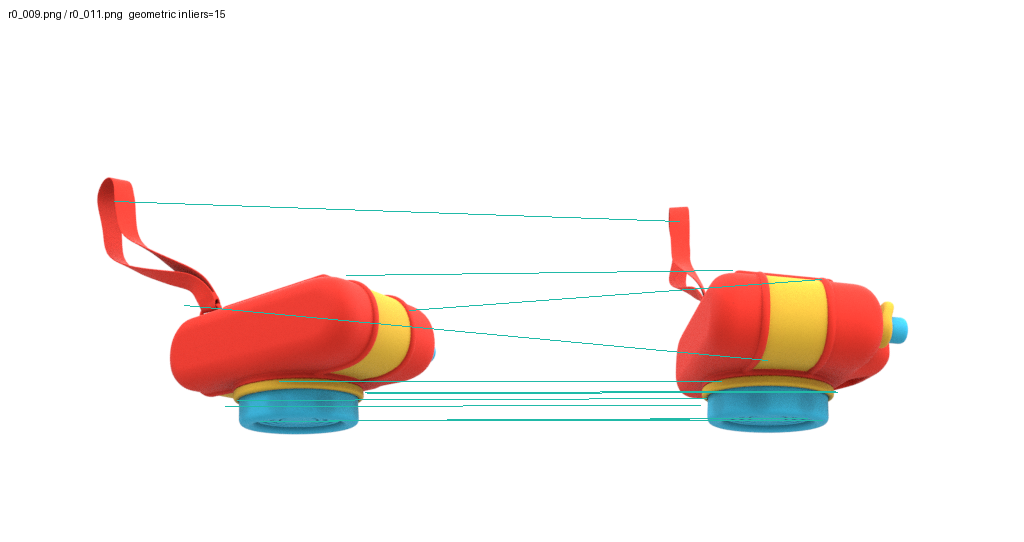
\includegraphics[width=\linewidth]{results/2891f204385c429eb8ab3cbc28bdf36a/matches/matches_00.png}\par
{\footnotesize PSNR 41.76 dB; foreground 32.49 dB.}\end{minipage}\hfill
\par\bigskip
\noindent\begin{minipage}[t]{0.48\linewidth}
\textbf{Cake}\par\smallskip
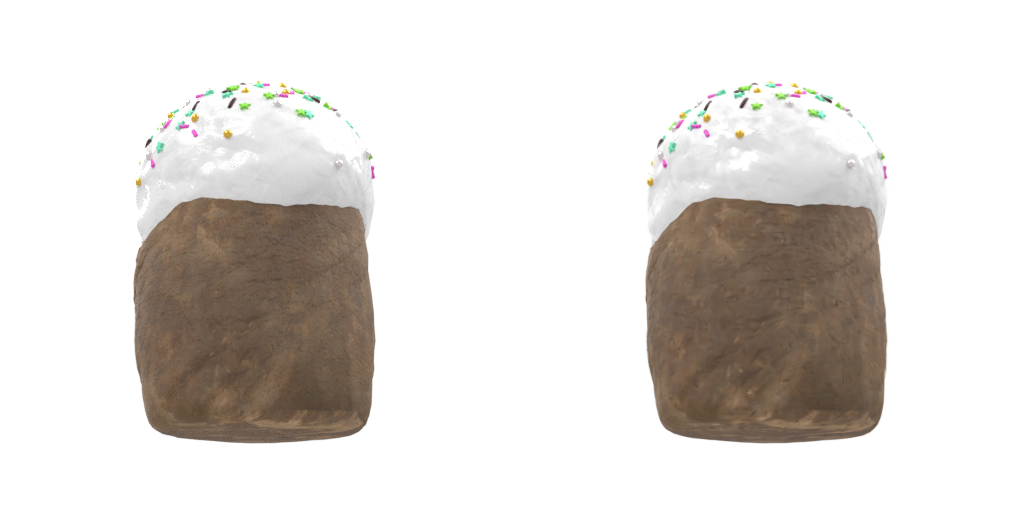
\includegraphics[width=\linewidth]{results/5fb6e07b6d864a4385c0018ed5f88010/evaluation/view_000.png}\par
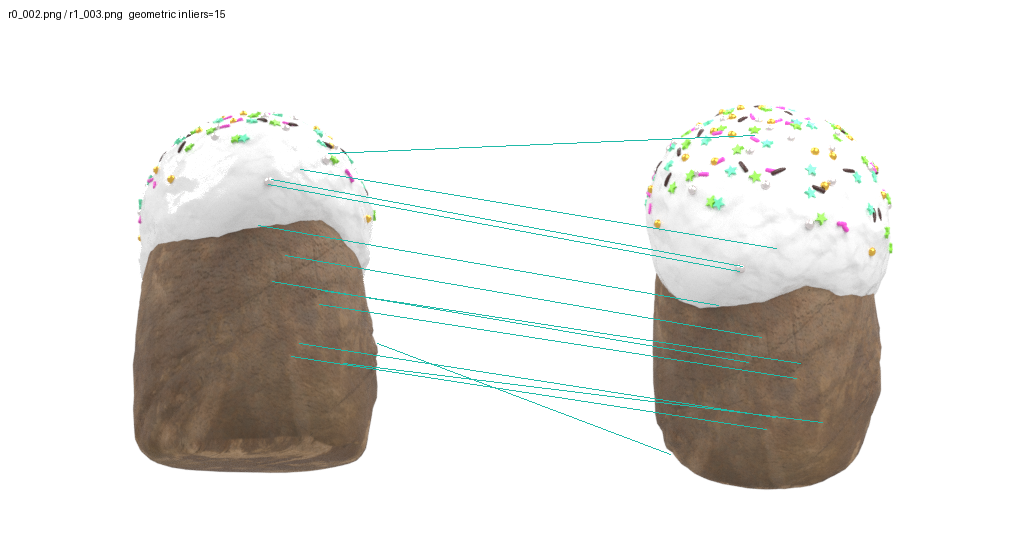
\includegraphics[width=\linewidth]{results/5fb6e07b6d864a4385c0018ed5f88010/matches/matches_00.png}\par
{\footnotesize PSNR 38.76 dB; foreground 31.67 dB.}\end{minipage}\hfill
\noindent\begin{minipage}[t]{0.48\linewidth}
\textbf{Garbage Bag}\par\smallskip
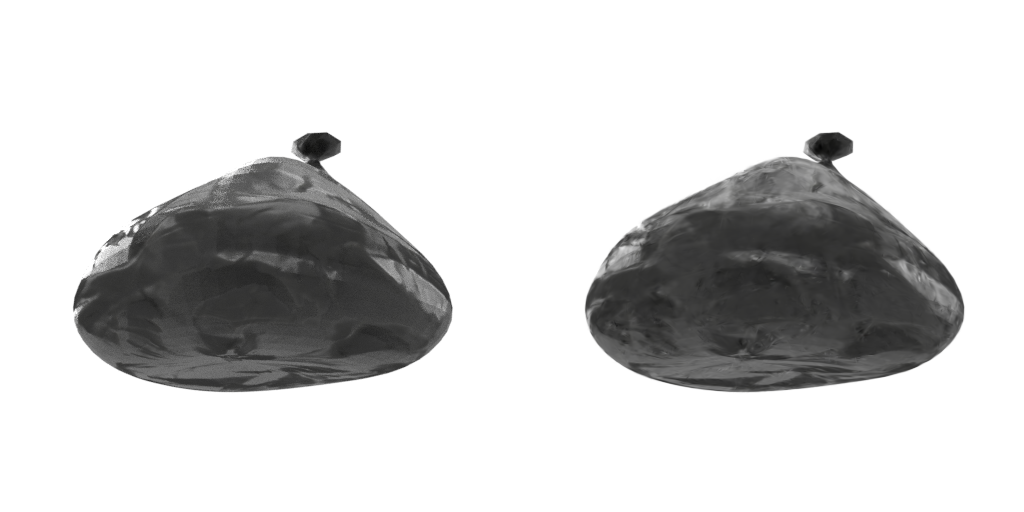
\includegraphics[width=\linewidth]{results/e0e9fb929170400c87c03c49a50ce315/evaluation/view_000.png}\par
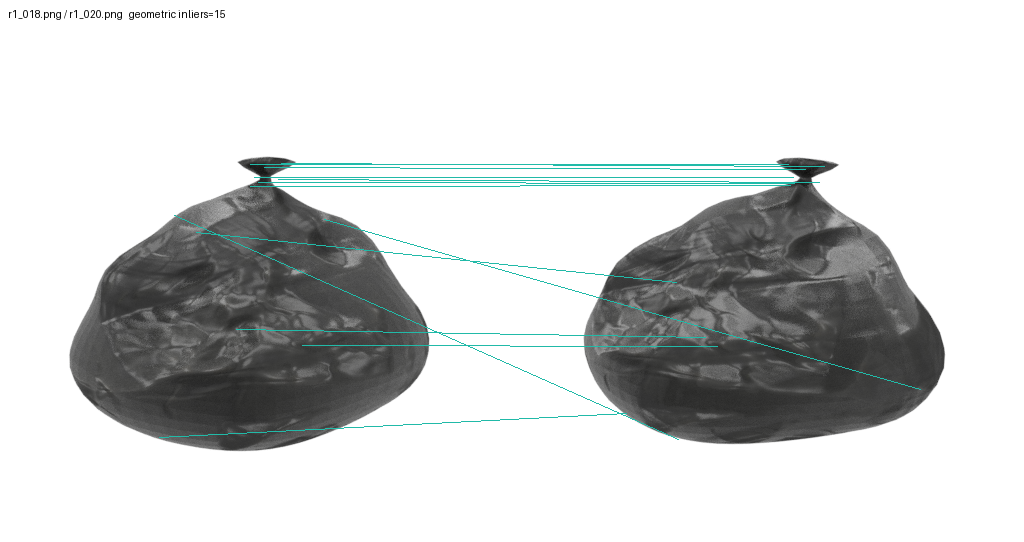
\includegraphics[width=\linewidth]{results/e0e9fb929170400c87c03c49a50ce315/matches/matches_00.png}\par
{\footnotesize PSNR 33.93 dB; foreground 28.59 dB.}\end{minipage}\hfill
\par\bigskip
\clearpage\section*{Reconstruction and matching evidence (3/3)}
Each object shows a held-out target (left) and a trained 3DGS rendering (right), followed by an actual geometrically verified matching pair. Full correspondences and looping GIFs are in the repository.\par\medskip\noindent\begin{minipage}[t]{0.48\linewidth}
\textbf{Globe sculpture, San Francisco}\par\smallskip
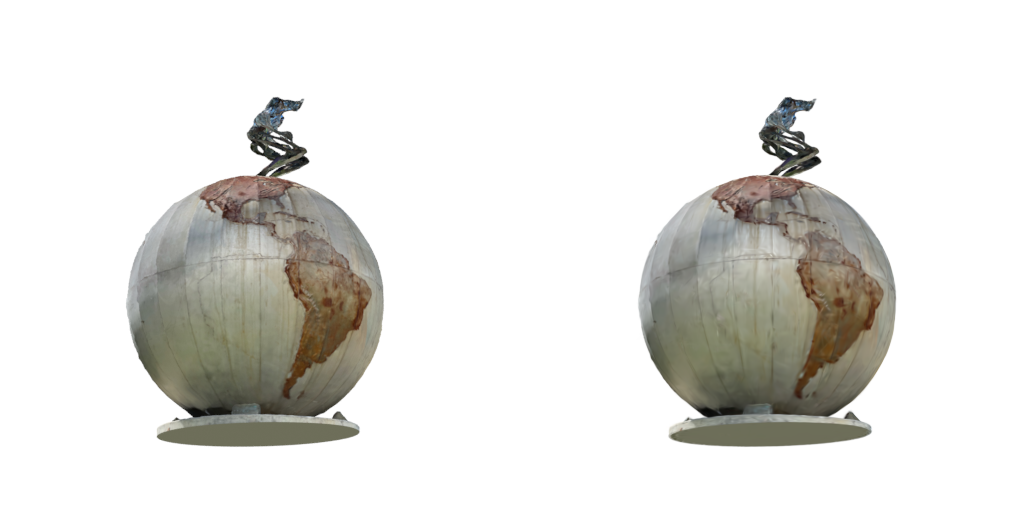
\includegraphics[width=\linewidth]{results/e843fbcdd9f746e2bca65e54f02a1845/evaluation/view_000.png}\par
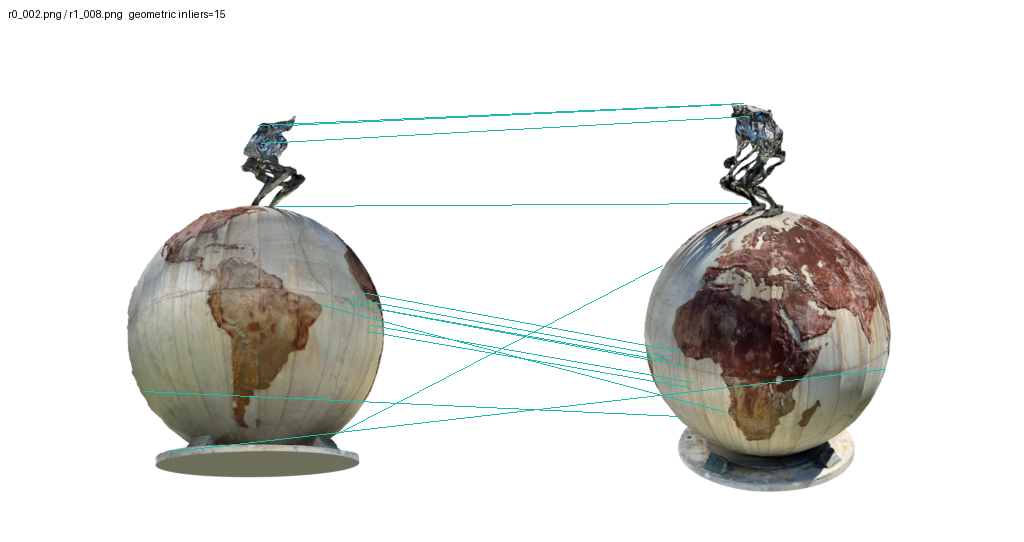
\includegraphics[width=\linewidth]{results/e843fbcdd9f746e2bca65e54f02a1845/matches/matches_00.png}\par
{\footnotesize PSNR 39.28 dB; foreground 32.79 dB.}\end{minipage}\hfill
\noindent\begin{minipage}[t]{0.48\linewidth}
\textbf{My First 3D Model - Guitar}\par\smallskip
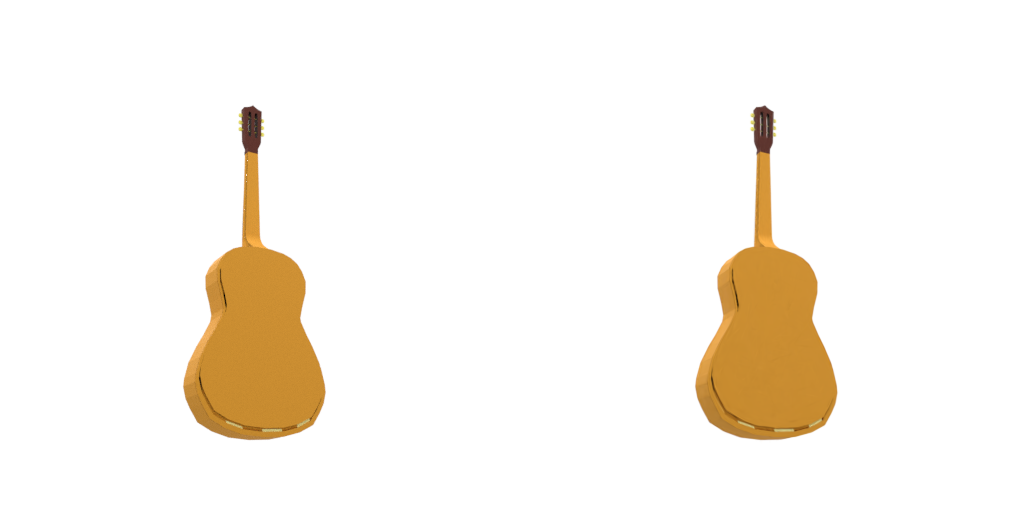
\includegraphics[width=\linewidth]{results/b3cb7a8487774fc28fa9702f8e36bb9d/evaluation/view_000.png}\par
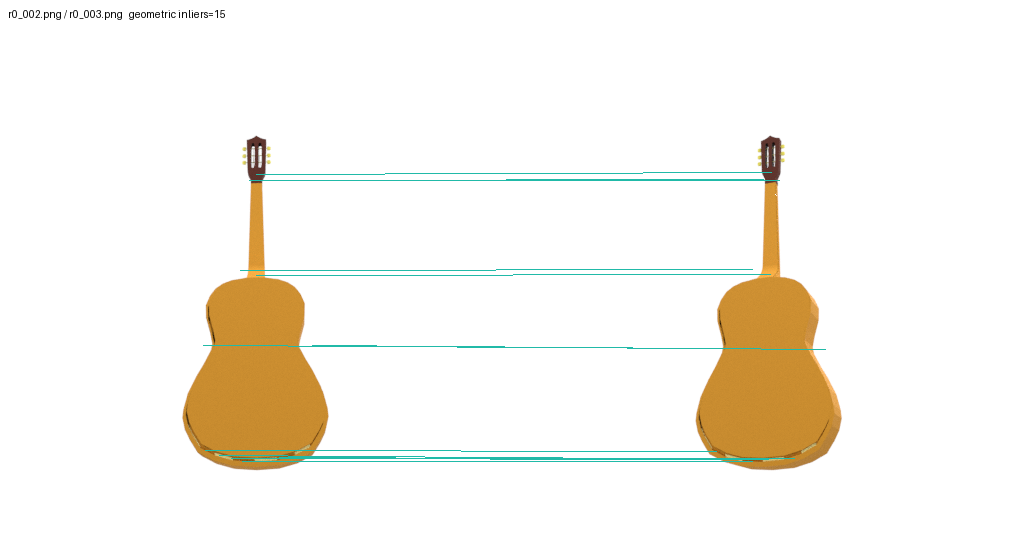
\includegraphics[width=\linewidth]{results/b3cb7a8487774fc28fa9702f8e36bb9d/matches/matches_00.png}\par
{\footnotesize PSNR 42.76 dB; foreground 30.75 dB.}\end{minipage}\hfill
\par\bigskip

\end{document}
